\documentclass[border=5mm,tikz,convert]{standalone}
\begin{document}
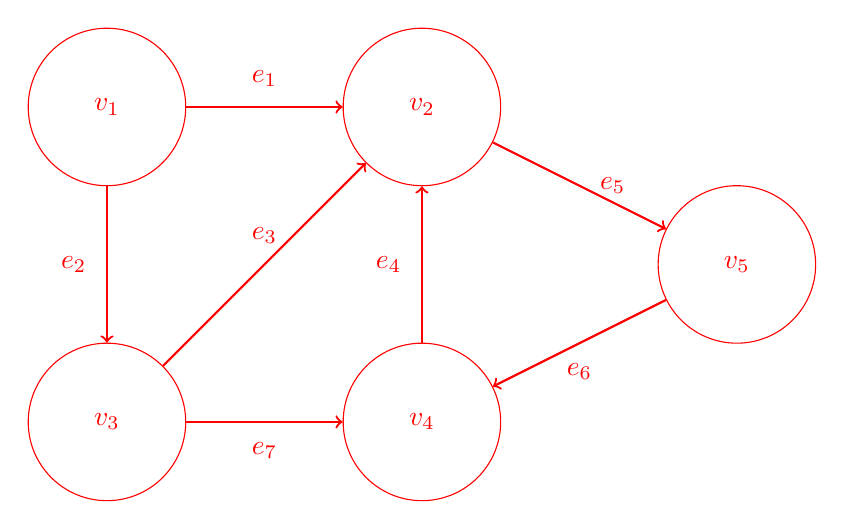
\begin{tikzpicture}[
nd/.style = {draw,circle,minimum size=2cm,red},
dedge/.style = {->, thick,red}
]
  \node[nd] (v3) at (0,0) {$v_3$};
  \node[nd] (v1) at (0,4) {$v_1$};
  \node[nd] (v2) at (4,4) {$v_2$};
  \node[nd] (v4) at (4,0) {$v_4$};
  \node[nd] (v5) at (8,2) {$v_5$};
  
  \draw[dedge] (v1) -- (v2) node [midway, label={$e_1$}] {};
  \draw[dedge] (v1) -- (v3) node [midway, label=left:{$e_2$}] {};
  \draw[dedge] (v3) -- (v2) node [midway, label=above:{$e_3$}] {};
  \draw[dedge] (v4) -- (v2) node [midway, label=left:{$e_4$}] {};
  \draw[dedge] (v2) -- (v5) node [midway, label=right:{$e_5$}] {};
  \draw[dedge] (v5) -- (v4) node [midway, label=below:{$e_6$}] {};
  \draw[dedge] (v3) -- (v4) node [midway, label=below:{$e_7$}] {};
\end{tikzpicture}
\end{document}
